\chapter{Introduction}

This file contains the script for the malware part of the SecureRole role-playing game.
It is intended to give you, the reader, a deeper understanding of the material and provide important additional information about malware.
\\

\begin{figure}[h!p]
    \centering
    \includegraphics[width=0.6\textwidth]{./images_malware/malware_screen}
    \label{img:malware_screen}
\end{figure}

In case that you played the role-playing game, you already know that we used the WannaCry malware (and if not, you know now).
This has a couple of reasons.

\begin{itemize}
    \item WannaCry was one of the first big ransomware attacks in Europe and the World%~\cite{BBCNews.13.May2017}
    \item The malware exploited a patched vulnerability, making it preventable
    \item It is a great example of how quickly malware can spread
    \item It proved to be devastating to large parts of its affected infrastructure
\end{itemize}

First of all, we will take a deeper dive into what exactly is malware and its subcategory ransomware, in which WannaCry falls.
Then we will take a deeper dive into WannaCry.
This includes how the attack played out, what exactly made the attack so successful and how it was stopped.
\\

If you want to learn more about WannaCry, we recommend this \href{https://www.techrepublic.com/article/wannacry-the-smart-persons-guide/}{cheatsheet} created by Tech Republic.
Or feel free to consult our \enquote{additional content} section for this topic, where we have placed many sources talking about WannaCry.
\\

%TODO ask Anina where additional content is stored!

\chapter{General Malware characteristics}

What exactly is malware?
Malware is a new word, which was created by combining \enquote{malicious} and \enquote{software} into one word.
As the name implies, this is a designation for any computer program that is intentionally designed to cause harm to a system.
You see how this designation is quite broad and is thus aimed at many of today's threats floating around the internet.
\\

Wikipedia lists 6 main types of malware%~\cite{Wikipedia.b}
, which are (in no particular order):

\begin{itemize}
    \item Trojan horses
    \item Rootkits
    \item Backdoors
    \item Infectious malware
    \item Ransomware
    \item Grayware
\end{itemize}

While all of these definitely deserve their own chapter, we will mainly cover ransomware (and to some extent infectious malware) in this script.
Nevertheless, we want to briefly introduce these six types of malware to understand what exactly they do and how they differ from ransomware.

\section{Trojan horse}

Trojan horses are like the historical horse of Troy, masquerading as something good while being of malicious intent.
Regarding malware, these programs usually pose as utilities such as antivirus software or tools.
They then secretly execute a payload, which can have many uses, such as keyloggers, backdoors or crypto miners.
This is done secretly so that neither the user nor any antivirus software notices that something malicious is happening on the system.

\section{Rootkits}

Rootkits are usually not a first stage of a malware attack, but rather the second stage.
They nest inside the operating system, where they alter its behavior to avoid detection by the operating systems malware countermeasures.

\section{Backdoors}

Backdoors are ways to access a system (often through an attached network) without the usual authentication.
Since these channels are rarely open by default, the malware creates such access points by disabling security features or opening new ways to access a system.
This can be used for different malicious purposes, such as stealing data, loading additional malware, or even using the computer as part of a botnet\footnote{Botnets are clusters of infected systems controlled by an entity and (usually) used for malicious purposes. It is estimated that the largest botnets included up to 30 million devices}.

\section{infectious malware}

Viruses and worms fall into this category.
And like their physical counterparts, they are designed to spread themselves, either on their own or with the help of other programs, to infect as many other systems as possible.
The main difference between the two is that a worm can spread without any interaction. A virus, on the other hand, requires user interaction (e.g., running infected software) to spread on a system.

\section{Ransomware}

A detailed account about ransomware is given in the next chapter, \autoref{sec:ransomware}.

\section{Grayware}

which is also more commonly known as spyware or adware, a program that performs a function and has undesirable aspects to it.
This could be a utility software, which shows advertisements during it's operation.
While this example is rather annoying, these types of programs can also be malicious, stealing user data and sending it to an attacker or weakening the computer's security.

\chapter{Ransomware}
\label{sec:ransomware}
\section{History}

Although malware and thus ransomware are not a new phenomenon, they have gained popularity in recent years.
This is mainly because before the introduction of cryptocurrencies, it was quite difficult to anonymously and efficiently extort ransom from victims around the world.
The introduction of cryptocurrencies allowed hackers to gather ransom in a semi-anonymous way with greater efficiency than ever before.
\\

This aided the rise of ransomware.
In the past, malware was mainly used to wreak havoc on a system, spy on users or create a powerful botnet.
But the attackers could now directly extort their victims without any additional steps.
An example, before ransomware, a hacker might send a trojan horse to a victim, which contained a keylogger.
They would then need to record what the victim was typing on its computer, scout this information for logins or banking information, and then use that information to break into a bank account to steal the victim's assets.
With ransomware, everything now happens in one step.
The machine gets infected with the ransomware, encrypts the user's file, and demands the ransom, without the hacker having to intervene once.
This adds a lot of comfort for a hacker, which can now collect his ransom in his preferred cryptocurrency and remain largely anonymous.
\\

This increase in convenience and anonymity caused ransomware usage to gradually rise, reaching new heights year after year.
The golden age for ransomware was on the rise.
%~\cite{DannyPalmer.October282021}
WannaCry then marked the first global ransomware attack, which disrupted services, brought companies' daily business to a halt and endangered the data of private individuals.
This marked a new era of malware.
\\

\section{Ransomware Types}

There are many ways to categorize ransomware, as it highly depends on which aspects are even taken into consideration.
Maybe one of the best categorizations was done in an article by Norton, in which they describe five most common types of ransomware%~\cite{Norton.November242021}.
\\

The types are:
\begin{itemize}
    \item Crypto-Ransomware
    \item Locker-Ransomware
    \item Scareware
    \item Ransomware as a Service (RaaS)
    \item Doxware/Leakware
\end{itemize}

\subsection{Crypto-Ransomware}

Crypto-Ransomware tries to encrypt all important files on a user's computer and then withhold the private key from them.
This key is then usually held for ransom, with the promise of decrypting the files for a user.
WannaCry was a crypto-ransomware in its core.

\subsection{Locker-Ransomware}

The locker-ransomware goes one step further and tries to lock the user out of the system, disabling all basic computer functions until the victims pays the ransom.
Usually, only a screen with the ransom note is accessible to the victim and nothing else.

\subsection{Scareware}

Scareware usually lacks the technical capabilities of the crypto and locker-ransomware and instead tries to scare the user into giving up the ransom payment.
This is usually done with fake claims about being monitored by a government organization, or having illegal files on one's machine.
They sometimes coerce the user into downloading more software (for example a fake antivirus software) which will then contain the main part of the ransomware, be it a locker or crypto-ransomware.

\subsection{Ransomware as a Service}

It is exactly what it says.
Cybercriminals perform ransomware attacks as a service to a paying customer.
This can be done for a variety of motives, such as money, destabilizing certain infrastructure, or harming competitors.

\subsection{Doxware/Leakware}

This ransomware usually steals the data it finds on an infected host, before possibly (but not necessarily) encrypting it.
The attacker then threatens to release the sensitive data to the public if the victim is unwilling to pay the ransom.

\chapter{WannaCry}

\begin{figure}[h!p]
    \centering
    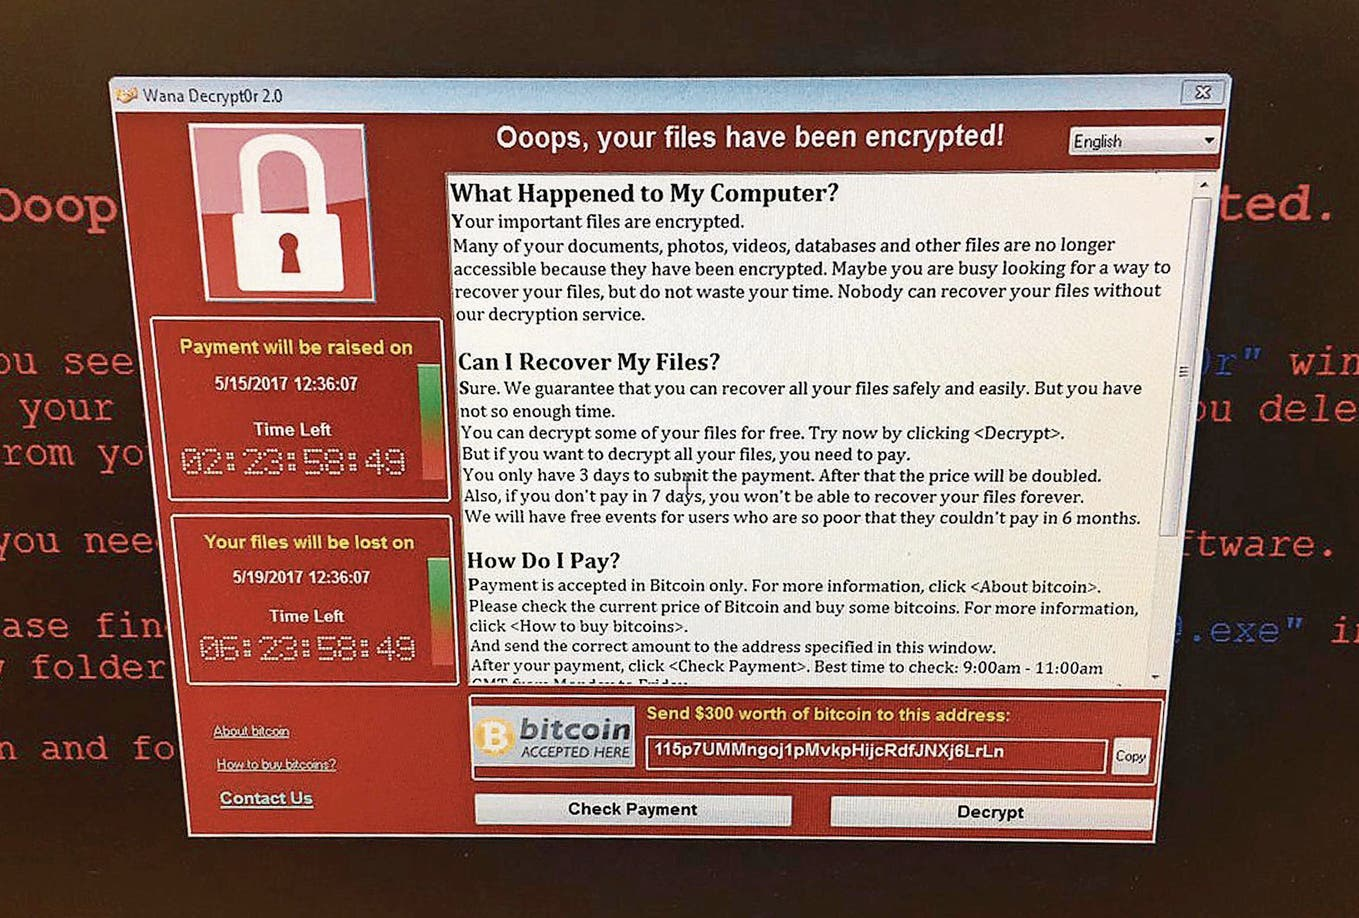
\includegraphics[width=0.6\textwidth]{./images_malware/WannaCry_screen_III.jpeg}
    \caption{The screen appearing, when a system is infected with WannaCry.}
    \label{img:wannacry}
\end{figure}

\section{Quick History}

The WannaCry attack started in the early morning on the 12th of May 2017, probably on the Asian continent.
It is believed that the initial compromise was due to a vulnerable %\acrshort{SMB} 
SMB port.
%~\cite{Wikipedia.}
It then quickly spread to 230'000 devices in 150 countries within the first day.
Luckily, the information technology researcher Marcus Hutchins%~\cite{Wikipedia.} 
discovered a kill switch domain \footnote{A domain, which tells the malware to be active or inactive. Often used to prevent an out of control spread, like an off switch.} which was hard-coded in the ransomware code.
\label{sec:killswitch}
He registered the domain name, creating a DNS sinkhole\footnote{A DNS Sinkhole is a Domain Name System Server which hands out addresses which can't be accessed, making a page inaccessible.}.
This action stopped all the spread of the ransomware on the 15th of May.
This was because the ransomware checked whether the domain was active before infecting a machine, which was the case now.
\\

This quick spread was attributed to a vulnerability of Microsoft operating systems, which it used to propagate.
The used vulnerability is called \enquote{EternalBlue}.
It exploits a weakness in the %\acrshort{SMB} 
SMB and thus allows the worm to remotely execute code on any victim machine.
This is all you need to know for now, we will take a closer look at this vulnerability in %\autoref{sec:Eternal_Blue}.
\\

The vulnerability had been developed by the NSA and leaked by an unknown hacking group, called the %\Gls{shadow}
shadow brokers, months prior to the WannaCry attack.
Microsoft had even released a patch to address the vulnerability for all currently supported operating systems
\footnote{That includes: Windows Vista, Windows 7, Windows 8.1, Windows 10, Windows Server 2008, Windows Server 2012, and Windows Server 2016}.
However, this meant that users who had not installed the patch or were still on unsupported operating systems were vulnerable to EternalBlue.
And as it turned out, many machines worldwide were affected.
\\

\section{Global reach}

WannaCry reached notoriety in Europe due to its significant disruptions in the UK healthcare system.
While the countries with the most infected systems were Russia, Ukraine, India and Taiwan, many European countries also suffered big disruptions.
It managed to take down medical equipment, such as MRI machines and blood refrigerators in the UK.
This caused major delays in the treatment of patients across the UK.
The reason for their overproportion outages was that a large portion of %\acrshort{NHS}
NHS hospitals were still running Windows XP, which had been discontinued since 2014\footnote{This is regarding the extended support, the mainstream support was shut down in 2009 already.}.
The use of medical equipment, believed to be incompatible with newer operating systems mandated the use of Windows XP.
\\

It furthermore disrupted public services in Europe and shut down production plants in the automotive industry, such as Renault in France.
Most companies were back online relatively quickly because they had sufficient backups and responded quickly to the crisis.
But at the same time, small private companies with inadequate cybersecurity and data backup measures were hit much harder.
\\

This issue was amplified because the malware was poorly written, and the attackers acted unprofessionally.
While this meant that recovering the files was often complicated and did not even happen after paying the ransom, it also meant that the damage could have been much worse.
Researchers remarked that would the malware had been more appropriately constructed and targeted, it could have caused significant disruptions in global infrastructure.
\\

The estimated economic losses by WannaCry reached 4 Billion USD.
%~\cite{Wikipedia.}

\section{Technical aspects}

As previously discussed, WannaCry used EternalBlue to infect machines and propagate in networks.
But this is far from the only vulnerability that it actually used.

\subsection{SMB}

The %\acrlong{SMB} 
SMB deserves its own mention in this section.
Don't be mistaken, the %\acrshort{SMB} 
SMB was not an attack, but it was crucial in the distribution of WannaCry, since it allowed for the creation of EternalBlue.
\\

The
%\acrshort{SMB} 
 SMB is a protocol developed by IBM and enhanced by Microsoft to allow devices shared access to files and printers across a network.
Due to this powerful use case of this protocol, security researchers and hackers have probed it for vulnerabilities many times in the past.
There have been many vulnerabilities that allowed attacks, one of the most prominent was EternalBlue.
\\

But even to this day %\acrshort{SMB} 
SMB is being tested, with the latest CVEs being discovered in 2020, for example the \href{https://nvd.nist.gov/vuln/detail/CVE-2020-1206}{SMBv3 information disclosure vulnerability}. 
\\

If you would like to know how the SMB works, we have this great \href{https://www.youtube.com/watch?v=csocwMe7l_E}{video} by NordVPN, which gives a quick overview.


\subsection{EternalBlue}
\label{sec:Eternal_Blue}

Eternal Blue was a vulnerability discovered and tracked by the NSA.
It allows for remote code execution on any vulnerable host, which is a great way of lateral movement in any Network.
While the NSA did not disclose this vulnerability, a hacker group which stole it from them did.
After the so-called %\enquote{\Gls{shadow}} 
 \enquote{shadow brokers} leaked the vulnerability, Microsoft managed to roll out a security patch which fixed it on all supported systems.

\subsection{Double Pulsar}
\label{sec:Double_Pulsar}

Double Pulsar is a backdoor vulnerability that, when installed on a system, allows elevation of privilege and thus code execution.
WannaCry used this to install a copy of itself on each machine it encountered and run it.
This vulnerability was also discovered and further pursued by the NSA and then subsequently leaked by the %\Gls{shadow}
 shadow brokers.
It was included in the EternalBlue security patch, rolled out by Microsoft.

\subsection{The procedure}
WannaCry would spread to a system and first check if the kill switch (see \autoref{sec:killswitch}) was active or not.
If it was inactive, it would encrypt all important files on the system.
Once that was done it would use the EternalBlue vulnerability and see if it could spread to machines on the same network.
The final step was to display the ransomware screen with a timer and the attackers' Bitcoin wallets.

\chapter{Prevention and Countermeasures}

When talking about how we can combat malware and ransomware we can divide the efforts taken into three main categories:
\begin{itemize}
    \item Prevention (Actions before the attack happens)
    \item Countermeasures (Actions during attack)
    \item Restoration (Actions after successful attacks)
\end{itemize}

The following sections will take a closer look at teach of those phases and will give a deeper look into how they are done.

\section{Prevention}

Due to the fact that preventing malware or ransomware attacks is quite similar, this section will always talk about \enquote{malware} even though it means both ransomware and malware.
\\

One of the most important steps in containing malware is not getting it on a system in the first place.
This can only be achieved by a strong prevention program.
While there are technical ways to do this, (see \autoref{sec:technical_countermeasures} ), the most important line of defense is the user.
\\

\subsection{The human firewall}

The users of a company are usually the firt ones to come in contact with the malware (after ingress filters and firewalls).
This is because one of the most common ways malware is spread is still spam e-mails, files with macros sent via e-mail, etc\dots.
All of these require human interaction to be effective and make it onto the target system.
\\

To keep your employees sharp and prepared, it is important to train them.
While the effectiveness of such trainings is debateable\footnote{A recent study conducted by ETH found that spam trainings are not as effective as previously hoped.
%~\cite{Lain.14122021}
If you want a good overview, TechRepublic released an article talking about the findings
%~\cite{CedricPernet.January132022}
}
they are the main measure for many companies to keep their users sharp.
The training helps employees know what current phishing e-mails look like and how they can easily spot them.
\\

This stops the malware attack dead in its tracks, since the malicious payload never gets executed and thus cannot reach the system.
\\

A further, often overlooked, part of the human firewall is quite simple.
Do not leave your devices unattended.
While this might not matter when you are leaving your laptop unlocked in a conference room, it starts an unhealthy habit.
Next time you might forget to lock it in a public library or your neighborhoods coffee shop.
All it takes is a malicious attacker, a rubber ducky \footnote{A rubber ducky, is a small computer which is often packaged to mimic the appearance of a computer. It is programmable and executes commands once it is plugged into your machine. This is done in rapid succession, so that it is impossible for a user to intervene, and sometimes even see what is going on until it is too late. They are often used in USB drop attacks or in public scenarios to quickly hijack computers.} and your system can already be compromised.
\\

This threat is also quite close to the next one.
Social Engineering.
While we do not want to completely open up this topic for you (since this thing also deserves a topic on it's own) it is an important mention.
Social Engineering is the act of persuading or pressuring other people into performing actions which they should not do.
While phishing is one form of social engineering, it can also take more advanced forms, such as phone calls asking users to reveal their credentials or simple face-to-face conversations persuading the person to insert a USB stick into their device.
Other malicious actors can use social engineering to gain access to your system to tamper with it, and thus compromise your system.
\\

While a well-trained user can help keep your system secure, they are still one of the biggest attack surfaces and vulnerable to many more attacks than just phishing.
Users can fall for things like vishing combined with phishing, USB drops, and other attacks that target your system.
But each of these topics deserves their own chapter.
Check out our repository to see if we have any of them in stock!
\\

\subsection{The *actual* Firewall}
\label{sec:technical_countermeasures}

But this can also be achieved with some technical solutions.
Spam filters are one of the most commonly used tools.
You can read more about all the technical marvels we came up with to stop spam.
They are listed in the spam script which you can find in this repository.
\\

They mainly employ different types of filters and check to verify that an e-mail is not spam.

\subsection{Further technical measures}

Further technical measures are mainly implemented in access restrictions to the company systems.
This is usually done through the use of firewalls, VPNs and other appliances such as intrusion prevention systems.
These keep malicious actors out of the system and prevent them from loading their malicious payloads directly onto the company systems.
Or, at the very least, they can alert the system administrator when such an attempt is made so he or she can respond appropriately.
\\

Another important aspect is the rigorous implementation of software updates.
As you saw before, WannaCry was only so successful because it used an already patched vulnerability, which was still unpatched on many systems.
They simply had an outdated operating system.
This could have been countered\footnote{Not all companies had this chance, since they were running operating systems which were past their end of life. But if you consider that safe practice in any company, your IT team needs to get back to the drawing board. Sadly, those institutions often have very limited IT budgets (Such as hospitals) and are thus prone to such oversights, since they simply lack the funds to replace aging hardware.} if the companies had kept their software up to date.

\section{Countermeasures}

While it is incredibly hard to keep malware and ransomware out of your system, the problems are really just starting once it infects one of your systems.
This has the clear advantage that it becomes detectable, but during the time it isn't detected, the malware can wreak havoc on your system.
Ranging anywhere from quietly propagating from machine to machine for future malicious purposes, up to directly taking machine after machine offline or even encrypting them, creating chaos.
\\

Malware detection is an important step in every companies defenses.
Thus, many commercial solutions have popped up over the years.
These have to be specially engineered, since modern malware usually uses evasion tactics to stay hidden on a system when it's spreading, limiting conventional antivirus effectiveness. %~\cite{KurtBaker.February42021}
So companies advise the users to keep an eye out if their system is behaving strangely, since this can usually be one of the earliest ways to detect if malware is propagating on the system.
\\

Once the malware starts to act up, modern EDR %Insert abbreviation for edr
solutions can pick it up and report it to the IT department.
EDR solutions are specifically engineered to pick up strange software behavior on machines, which a classical antivirus usually is not capable of doing.
%~\cite{Trellix.}
Now a quick response is necessary to make sure the malware has no time to destroy important company property.

\section{Removal}

One of the most important things, during the removal and restoration process is, that even though this is time critical in most cases, you sit down and develop a plan.
Many companies, including SANS \footnote{Sans has released an \enquote{Incident Handler's Handbook} which you can download at this \href{https://www.sans.org/white-papers/33901/}{address}. }%Abbr
and the NIST \footnote{The NIST has pusblished their work under the following \href{http://dx.doi.org/10.6028/NIST.SP.800-61r2}{Link}. }%Abbr 
 have developed standard procedures on how to tackle a ransomware cases.
It is important that think about which devices on your network are infected, how you plan to remove the malware from them, and which you will restore.
So that you can later focus on a speedy recovery, and not lose time due to administrative errors, which can in turn lead to more work later on.
\\

While some aspects of these plans are tailored to the malware you are facing, it is always a good idea to have read and understood these documents \textbf{before an incident occurs}.
They help you to put measures in place to prepare for similar attacks.
It drastically reduces your response time if you already have procedures in place before an incident occurs.
\\

So now the malware needs to be removed from the system, but how can we go about this without destroying important data?
A malware infection has many similarities to a medical condition.
The sooner you can determine what is the cause, the faster and easier will be your response.
So not all removal techniques can be used in all situations.
\\

If the infection is just starting, the removal is fairly easy.
A good antivirus solution that is tailored to spotting and removing malware can quarantine it or remove it from your system, without much user input needed.
\\

Should the antivirus solutions be overwhelmed with the malware, we need more drastic measures.
There are special tools which are designed to remove malware.
These can be launched from an external device, such as a flash drive to skip the installation, which would often be thwarted by the malware itself.
The list of companies which create such solutions is long, so you will find something for your exact use case.
\\

But what if your system is fully encrypted?
Or locked?

\section{Restoration}

Then you have no choice left but to go into the restoration phase.
This phase is usually the last step in any malware removal process, no matter if you successfully managed to get rid of the malware or not.
\\

If your system is encrypted or locked, you still have a chance of restoring it and regaining access to your data.
One of the most well known ways to do this, is by visiting the \href{https://id-ransomware.malwarehunterteam.com}{webpage of the malware hunter team}.
They are a small group of ransomware researches who upload known solutions developed by other security researches or themselves, which allow victims of ransomware to restore their data.
This is only possible with malware that has already been cracked, so there is a chance that the malware that attacked you is too new to be found on this website (should you ever seriously be attacked by malware).
\\

So what if there is no option left?
Your data is encrypted, there is no decryptor available and your antivirus has died?
\\

Backups.
\\

Your last resort should be wiping the system, running through a clean setup (best done air gapped as to not be reinfected, should the malware still be lingering on your network.)
This is critical.
Because even if you do everything right, an infected machine that you might not even think about (such as a printer, a dormant server, etc.) could still contain the ransomware, and once your new clean machine connects to the network, it will be reinfected, and the whole process needs to start over.
\\

Then when the process of restoring the clients is completed, and you copied all the backups onto the clients, you can slowly begin to rebuild the system in its entirety.
This can usually not be done ad-hoc and needs meticulous preparations, such as a list of all infected hosts, what needs to be restored and removed and which backups need to be loaded on which hosts.
\\

The process of using backups should also be rehearsed.
If it's the first time you use them, when you are reacting to an attack, chances are high that something will misfire, a backup will not work, or you are simply overwhelmed by the amount of work necessary to install backups.
All of this can still happen when you are properly trained for it, but the chances are more in your favour if the whole task is a little more routine.

This is one of the reasons, why we previously urged you to set up a strategy to deal with the ransomware, or really any attack.
\chapter{Questions}

Thank you for taking the time to read through this script.
We will now give you the opportunity to test the knowledge you have gathered with a few questions.
Should you not remember a question from the top of your head, feel free to go back a few pages and search for the solution.
All questions can be answered by reading this document, no additional reading of the source material or the mentioned additional material is necessary (but highly recommended).

\begin{question}[Question]
    Is all malware ransomware?\\
    Is all ransomware malware?\\
    Explain your answer.
\end{question}

\begin{question}[Answer]
    \vspace{3cm}
\end{question}


\begin{question}[Question]
    What are the two main categories described in infectious malware?\\
    What sets them apart from one another?
\end{question}

\begin{question}[Answer]
    \vspace{3cm}
\end{question}


\begin{question}[Question]
    What was one of the most important factors for the increase in popularity of ransomware?
\end{question}

\begin{question}[Answer]
    \vspace{3cm}
\end{question}


\begin{question}[Question]
    
    Was WannaCry fully preventable?\\
    If yes how so?\\
    If no, why not?\\

\end{question}

\begin{question}[Answer]
    \vspace{3cm}
\end{question}

\begin{question}[Answer]
    \vspace{3cm}
\end{question}

\begin{question}[Question]
    
    Do you think WannaCry was a well-executed attack?\\
    Explain why you feel this way.

\end{question}

\begin{question}[Answer]
    \vspace{3cm}
\end{question}

\begin{question}[Question]
    
    What made WannaCry stand out from other ransomware attacks at the time?\\
    What made it unique?

\end{question}

\begin{question}[Answer]
    \vspace{3cm}
\end{question}